\documentclass[11pt]{article}
\usepackage{amsfonts,amsmath,amssymb,amsthm} % Math packages
\usepackage{graphicx} % For including images
\usepackage{titlesec} % For customizing section titles
\usepackage{titling} % For customizing the title
\usepackage{geometry} % For adjusting page margins
\usepackage{datetime} % For formatting the date
\usepackage{hyperref} % For adding hyperlinks


% Customize the title format
\pretitle{\begin{center}\Large\bfseries}
\posttitle{\par\end{center}}
\preauthor{\begin{center}\large}
\postauthor{\end{center}}
\predate{\begin{center}\large}
\postdate{\par\end{center}}

% Customize the section title format
\titleformat{\section}{\large\bfseries}{\thesection.}{0.5em}{}

% Adjust the page margins
\geometry{margin=1in}

\begin{document}

% Create the title page
\begin{titlepage}
    \centering
    \vspace*{0.5cm}
    \par\normalfont\fontsize{35}{35}\sffamily\selectfont
    Assignment 02 - MATH 525\par 
    \vspace*{1cm}
    {\huge\bfseries Huzaifa Unjhawala \\  Gabe Selzer \par} 
    \vspace*{1cm}
    {\Large\itshape Date: \today\par} 
    \vfill
\end{titlepage}

\tableofcontents
\newpage

\section*{Problem 1}
\subsection*{a} Let's check if each of the vectors is a basic solution : \\
For vector (0.5,1,0.5,0,0) we first check if it satisfies $Ax = b$ \\
\[-0.5 + 1 + 0.5 + 2(0) - 2(0) = 1\]
\[3(0.5) + 2(1) + 7(1/2) - 0 +4(0) = 7\]
\[-2(0.5) + 4(1) +6(0.5) +2(0) - 0 = 6\]
Thus, all the equality constraints are satisfied. Now we check if the columns corresponding to the basic-variables are linearly independent. We thus have the bases 
\[B  =  \begin{bmatrix}
-1 & 1 & 1  \\
3 & 2 & 7 \\
-2 & 4 & 6 
\end{bmatrix}\]
The columns of $B$ are linearly independent if $det(B) \ne 0$. However $det(B) = 0$. Thus, (0.5,1,0.5,0,0) is \textbf{NOT} a basic solution. Since its not basic it is also \textbf{NOT} degenerate.

Now, for vector (1,2,0,0,0), we follow the same procedure to see if $Ax = b$:\\
\[-1 + 2 = 1\]
\[3 + 2(2) = 7\]
\[-2 + 4(2) = 6\]
Thus $Ax = b$ is satisfied. This vector can potentially have 3 bases
\[B_1  =  \begin{bmatrix}
    -1 & 1 & 1  \\
    3 & 2 & 7 \\
    -2 & 4 & 6 
    \end{bmatrix}\]
\[det(B_1) = 0\]

\[B_2  =  \begin{bmatrix}
    -1 & 1 & 2  \\
    3 & 2 & -1 \\
    -2 & 4 & 2 
    \end{bmatrix}\]
\[det(B_2) = 20\]

\[B_3  =  \begin{bmatrix}
    -1 & 1 & -2  \\
    3 & 2 & 4 \\
    -2 & 4 & -1 
    \end{bmatrix}\]
\[det(B_3) = -19\]
Thus, the vector is a basic solution as it has atleast one valid basis in $\mathbb{R}^3$. According to \textit{Defination 2.11}, a basic solution is degenerate if more than $n-m$ components of the basic solution are zero. In this case $n = 5$ and $m = 3$. We have $ > 2$ zeroes, thus the vector is degenerate.\\

Finally, for vector (1,0,0,1,0) we see that it does not satisfy $Ax = b$
\[3(1) + 2(0) + 7(0) -1(1) +4(0) = 2 \ne 7\]
Thus, it is \textbf{NOT} a basic solution and is also \textbf{NOT} degenerate.

\subsection*{b}
Vector (0.5,1,0.5,0,0) and vector (1,0,0,1,0) are not basic solutions. Thus, according to \textit{Theorem 2.3}, they are not verticies. \\
Vector (1,2,0,0,0) is a vertex as its a basic solution. \\
Consider the cost function $c = \sum_{i \in I(x^*)} a_i$ where $I(x^*)$ is all the constraints active at $x^*$ and $a_i$ is the set of all cosntraints. This corresponds to, 

\begin{table}[h]
    \centering
    \begin{tabular}{|c|c|c|c|c|}
    \hline
    \textbf{$x_1$} & \textbf{$x_2$} & \textbf{$x_3$} & \textbf{$x_4$} & \textbf{$x_5$}\\ \hline
    -1 & 1 & 1 & 2 & -2 \\ 
    3 & 2 & 7 & -1 & 4 \\ 
    -2 & 4 & 6 & 2 & -1 \\ 
    0 & 0 & 1 & 1 & 1 \\ \hline
    $0x_1$ & $7x_2$ & $15x_3$ & $4x_4$ & $2x_5$ \\ \hline
    \end{tabular}
    \end{table}
With $\mathbf{c^T = [0,7,15,4,2]}$ and $x^{*T} = [1,2,0,0,0]$, we get $c^Tx^* = 14$. Since, $x^*$ is a basic feasible solution, \textit{Theorem 2.2 (c)} says that $x^*$ is the uniqure solution to $\{ a_{i}^T x = b_i | i \in I(x^*)\}$, thus all other feasuble $x$ have $c^T x \ne c^T x^*$ and $a_{i}^T x > b_i$ for some $i \in I(x^*)$. Thus $c^T x > c^T x^*$.


\section*{Problem 3}
\subsection*{a}

We first consider the case where $m\geq n$. In this case, for any $y=\sum_{i=1}^n\lambda_iA_i$ such that $y\in C$, even if \textbf{all} $n$ coefficients are nonzero, this is still $m$ or fewer nonzero coefficients.

The only non-trivial case to consider is when $m<n$. Consider some $y\in C$. By definition, $\exists \lambda_1, \cdots, \lambda_n\geq 0:y=\sum_{i=1}^n\lambda_i A_i$. There may, in fact, be multiple distinct $\lambda$, and we can define these $\lambda$ using the polyhedron $Q$:

$$
Q=\bigl\{(\lambda_1, \cdots,\lambda_n)\in\mathbb{R}^n:y=\sum_{i=1}^n\lambda_iA_i, \lambda_1, \cdots, \lambda_n \geq 0\bigr\}
$$
We notice that we can rewrite the condition $\sum_{i=1}^n\lambda_iA_i=y$ to the condition $y=A\lambda$:

$$
Q=\bigl\{\lambda\in\mathbb{R}^n:A\lambda=y, \lambda\geq 0\bigr\}
$$

This is then the standard-form polyhedron that we are very familiar with. We are given no information about the vectors $\{A_1,\cdots, A_n\}$, but we know that rank($A$)$=k\leq m$ must hold due to the number of elements in each vector. 

If $k<m$, then we could use Theorem 2.5 from the lecture notes to construct an equivalent polyhedron $Q'$, continue the proof using $Q'$ instead of $Q$, and develop a solution $Q'$ that, because Theorem 2.5 guarantees $Q'=Q$, also satisfies the constratints of $Q$. And, instead of having at most $m$ non-zero coefficients, that solution would have at most $k<m$ non-zero coefficients, satisfying the constraints of the problem. 

Thus, \emph{without loss of generality}, we assume that rank($A$)$=m$. Consider Theorem 2.4 from the lectures:

\bigskip

\noindent\fbox{%
    \parbox{\textwidth}{%
        Theorem 2.4
        
        Consider the constraints $Ax=b$ and $x\geq 0$ and assume that the $m\times n$ matrix $A$ has linearly independent rows. A vector $x\in \mathbb{R}^n$ is a basic solution if and only if we have $Ax=b$, and there exist distinct indices $B(1),\cdots, B(m)\in\{1,\cdots,n\}$ such that:
\begin{itemize}
\item The columns $A_{B(1)}, \cdots, A_{B(m)}$ of $A$ are linearly independent.
\item If $i\neq B(1),\cdots, B(m)$, then $x_i=0$.
\end{itemize}
    }%
}

Since $A$, a $m\times n$ matrix of rank $m$, has linearly independent rows, there must exist some set of $m$ linearly independent columns $A_{B(1)},\cdots, A_{B(m)}$ at indices $B(1),\cdots, B(m)$. We construct

$$
B=\begin{bmatrix}
A_{B(1)} & \cdots & A_{B(m)} \\
\end{bmatrix}
$$

We then define $\lambda_B=B^{-1}y$ (note that $B^{-1}$ exists since $B$'s columns are linearly independent), and
$$
\lambda_i^* = \begin{cases}
(\lambda_B)_j\quad \text{if }\exists B(j):i=B(j), 1\leq j\leq m\\
0\quad\quad\quad i\neq B(1), \cdots, B(m)
\end{cases}
$$
is a basic (feasible) solution in $Q$ conforming to Theorem 2.4. Since $\lambda^*\in Q$, by the definiton of $Q$ we have $y=\sum_{i=1}^n\lambda_i^*A_i$. Furthermore, since the first case of $\lambda_i^*$ applies at $m$ indices, there can be \textbf{at most} $m$ non-zero elements in $\lambda^*$. Thus we have shown that for any $y\in C$, we can find the required $\lambda_1,\cdots, \lambda_n$, namely our $\lambda^*$. Q.E.D

\subsection*{b}

We first consider the case where $m+1\geq n$. In this case, for any $y=\sum_{i=1}^n\lambda_iA_i$ such that $y\in C$, even if \textbf{all} $n$ coefficients are nonzero, this is still $m+1$ or fewer nonzero coefficients.

The only non-trivial case to consider is when $m+1<n$. Consider some $y\in C$. By definition, $\exists \lambda_1, \cdots, \lambda_n\geq 0:y=\sum_{i=1}^n\lambda_i A_i$. There may, in fact, be multiple distinct $\lambda$, and we can define these $\lambda$ using the polyhedron $Q$:

$$
Q=\bigl\{(\lambda_1, \cdots,\lambda_n)\in\mathbb{R}^n:y=\sum_{i=1}^n\lambda_iA_i, \sum_{i=1}^n\lambda_i=1, \lambda_1, \cdots, \lambda_n \geq 0\bigr\}
$$
We notice that we can rewrite the condition $\sum_{i=1}^n\lambda_iA_i=y$ to the condition $y=A\lambda$:

$$
Q=\bigl\{\lambda\in\mathbb{R}^n:A\lambda=y, \sum_{i=1}^n\lambda_i=1, \lambda\geq 0\bigr\}
$$
We can then append our final equality constraint to create a new $(m+1)\times n$ contstraint matrix $\bar{A}$ and a single vector $\bar{y}\in\mathbb{R}^{m+1}$:
$$
\bar{A}=\begin{bmatrix}
A\\
\begin{bmatrix}
1&1&\cdots&1
\end{bmatrix}
\end{bmatrix}, 
\bar{y} = \begin{bmatrix}
y\\
1
\end{bmatrix}
$$
Thus we have:

$$
Q=\bigl\{\lambda\in\mathbb{R}^n:\bar{A}\lambda=\bar{y}, \lambda\geq 0\bigr\}
$$

This is then the standard-form polyhedron that we are very familiar with. We know that rank($\bar{A}$)$=k\leq m+1$ must hold due to the number of elements in each vector. 

If $k<m+1$, then we could use Theorem 2.5 from the lecture notes to construct an equivalent polyhedron $Q'$, continue the proof using $Q'$ instead of $Q$, and develop a solution $Q'$ that, because Theorem 2.5 guarantees $Q'=Q$, also satisfies the constratints of $Q$. And, instead of having at most $m+1$ non-zero coefficients, that solution would have at most $k<m+1$ non-zero coefficients, satisfying the constraints of the problem. 

Thus, \emph{without loss of generality}, we assume that rank($\bar{A}$)$=m+1$. Consider Theorem 2.4 from the lectures:

\bigskip

\noindent\fbox{%
    \parbox{\textwidth}{%
        Theorem 2.4
        
        Consider the constraints $Ax=b$ and $x\geq 0$ and assume that the $m\times n$ matrix $A$ has linearly independent rows. A vector $x\in \mathbb{R}^n$ is a basic solution if and only if we have $Ax=b$, and there exist distinct indices $B(1),\cdots, B(m)\in\{1,\cdots,n\}$ such that:
\begin{itemize}
\item The columns $A_{B(1)}, \cdots, A_{B(m)}$ of $A$ are linearly independent.
\item If $i\neq B(1),\cdots, B(m)$, then $x_i=0$.
\end{itemize}
    }%
}

Since $\bar{A}$, a $(m+1)\times n$ matrix of rank $(m+1)$, has linearly independent rows, there must exist some set of $(m+1)$ linearly independent columns $\bar{A}_{B(1)},\cdots, \bar{A}_{B(m)}$ at indices $B(1),\cdots, B(m+1)$. We construct

$$
B=\begin{bmatrix}
\bar{A}_{B(1)} & \cdots & \bar{A}_{B(m+1)} \\
\end{bmatrix}
$$

We then define $\lambda_B=B^{-1}y$ (note that $B^{-1}$ exists since $B$'s columns are linearly independent), and
$$
\lambda_i^* = \begin{cases}
(\lambda_B)_j\quad \text{if }\exists B(j):i=B(j), 1\leq j\leq m+1\\
0\quad\quad\quad i\neq B(1), \cdots, B(m)
\end{cases}
$$
is a basic (feasible) solution in $Q$ conforming to Theorem 2.4. Since $\lambda^*\in Q$, by the definiton of $Q$ we have $\bar{y}=\sum_{i=1}^n\lambda_i^*\bar{A_i}$, which then implies that $y=\sum_{i=1}^n\lambda_iA_i$ \textbf{and} $\sum_{i=1}^n\lambda_i=1$. Furthermore, since the first case of $\lambda_i^*$ applies at $m+1$ indices, there can be \textbf{at most} $m+1$ non-zero elements in $\lambda^*$. Thus we have shown that for any $y\in C$, we can find the required $\lambda_1,\cdots, \lambda_n$, namely our $\lambda^*$. Q.E.D


\section*{Problem 4}
For this question, we need to prove

\[ \{\lambda u + (1-\lambda) v | \lambda \in [0,1] \} = \{z \in P | a_{i}^{'}z =  b_i, i = 1,....n\} \]
in both directions. Let the set in the LHS of the above equation be $L_1$ and the set in the RHS be $L_2$. Thus we need to prove $L_1 \subseteq L_2$ and $L_2 \subseteq L_1$. 

\underline{$\mathbf{L_1 \subseteq L_2}$} \\

Let $z \in L_1$, then $z = \lambda u + (1 - \lambda) v$ where $u$ and $v$ $\in P$. Since $P$ is a polyhedron made by the intersection of convex hyperplanes, it is also convex. Thus, the line joining two points $u$, $v$ $\in P$ also $\in P$. \\
Also, consider a set of vectors $a_i \in \mathbb{R}^n$ where $i = 1,2,...n-1$, then, 
\[ a_{i}^T z = a_{i}^T \lambda u + a_{i}^T (1 - \lambda)v \]
\[ = \lambda a_{i}^T u + (1-\lambda)a_{i}^T v\] 
We know that , $a_{i}^T u = a_{i}^T v = b_i$ \\
\[ = \lambda b_i + (1-\lambda) b_i\]
\[ = b_i \]
as $\lambda \in [0,1]$. Thus $z \in P$ and $a_{i}^T z = b_i$ for $i=1,2,...n-1$. Thus the first $(n-1)$ constraints hold. For the remaining $(m-n)$ constrains $a_{i}^T u \ge b_i$ and $a_{i}^T v \ge v$, we note that since $u,v \in P$ , $a_{i}^T x = \lambda a_{i}^T u + (1 - \lambda) a_{i}^T v \ge \lambda b_i + (1-\lambda) b_i$. Thus, $L_1 \subseteq L_2$\\

\underline{$\mathbf{L_2 \subseteq L_1}$} \\

We know that $a_1,\cdots,a_{n-1}$ are linearly independent. Therefore, since each constraint $a_i'x=b_i$ describes a hyperplane in $\mathbb{R}^n$, each of the $n-1$ constraints $a_i'x=b_i, i=1,\cdots, n-1$ superimposed yields a $n-(n-1)=1$ dimensional space (line) in $\mathbb{R}^n$. We describe this space using $G$.

$$
G = \{ z \in \mathbb{R}^n : a_{i}' z = b_i, i = 1,2,...n-1\}
$$
Consider any vector $z\in L_2$. By the definition of $L_2$, it is also true that $z\in G$. By the definition of $u$ and $v$, we also know that $u,v\in G$.

Consider $(u-v)$. This vector is orthogonal to all vectors $a_i, i=1,\cdots, n-1$, as $a_i(u-v)=a_iu-a_iv=b_i-b_i=0$. Therefore, $(u-v)$ must be parallel to the line described by $G$, and from any point on $G$ we could add $c(u-v), c\in\mathbb{R}$ to that point to obtain \textbf{any point $z\in G$}. Thus we can describe any $z\in G$ as $z=v+\lambda(u-v)$. Thus we have $G=\{z\in\mathbb{R}^n|z=v+\lambda(u-v)\}$. We note that $L_2$ is the subset of $G$ containing items that are \emph{also} in $P$, i.e. $L_2=\{z\in P|z=v+\lambda(u-v)\}$. \\

\begin{figure}[h]
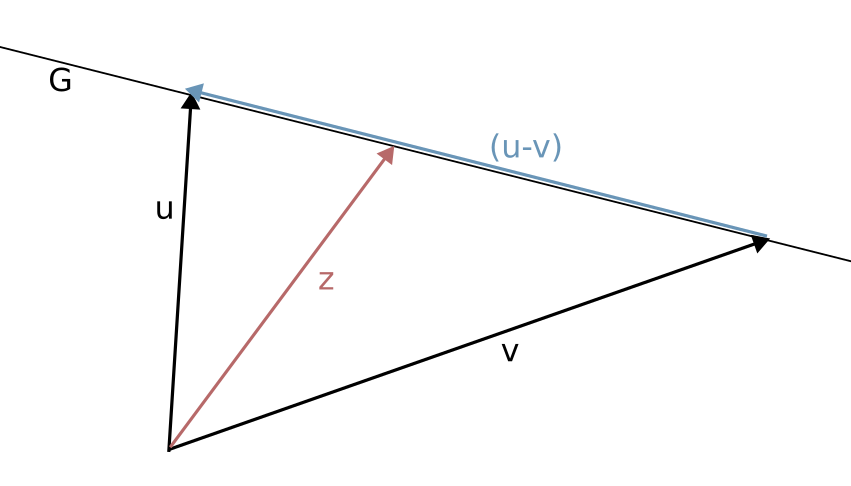
\includegraphics[width=0.5\textwidth]{4b-general}
\centering
\caption{A 1-dimensional representation of $u$, $v$, $z$, $G$, and $(u-v)$}
\end{figure}

All that remains is to show that $\{z\in P|z=v+\lambda(u-v)\}=\{\lambda u + (1-\lambda) v; \lambda\in[0,1]\}$ Consider $\lambda$:

\underline{$\lambda < 0$} \\

Suppose there exists some $z\in P$ such that $\lambda < 0$. This situation is shown in Figure 2. Note that in this case, $v$ is on the line segment between $u$ and $z$. By definition, this means that $v$ is not an extreme point, reaching a contradiction. Therefore $\forall z=v+\lambda(u-v)|\lambda<0$, $z$ is not in $P$.

\begin{figure}[h]
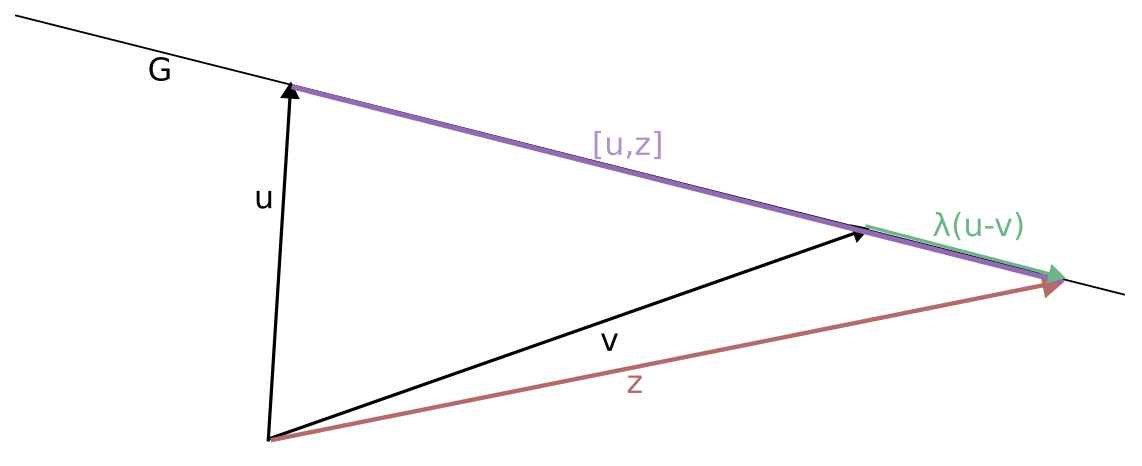
\includegraphics[width=0.5\textwidth]{4b-negative}
\centering
\caption{A 1-dimensional representation of $z=v+\lambda(u-v); \lambda<0$}
\end{figure}

\underline{$\lambda > 1$} \\

Suppose there exists some $z\in P$ such that $\lambda > 1$. This situation is shown in Figure 2. Note that in this case, $u$ is on the line segment between $v$ and $z$. By definition, this means that $u$ is not an extreme point, reaching a contradiction. Therefore $\forall z=v+\lambda(u-v)|\lambda>1$, $z$ is not in $P$.

\begin{figure}[h]
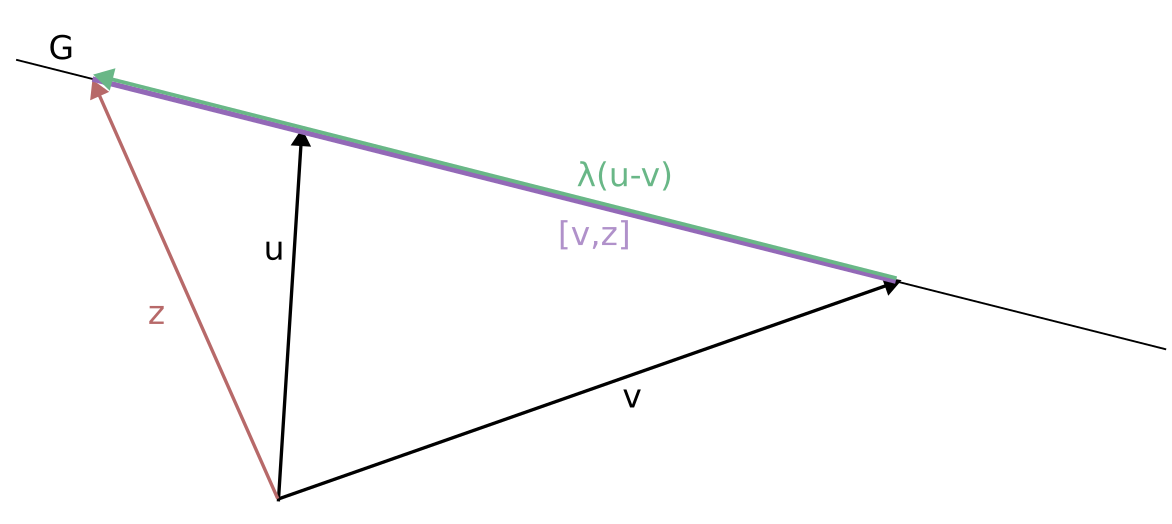
\includegraphics[width=0.5\textwidth]{4b-positive}
\centering
\caption{A 1-dimensional representation of $z=v+\lambda(u-v); \lambda>1$}
\end{figure}

Therefore, if $z\in P$, it must hold that $\lambda>0$ and $\lambda < 1$, and we can rewrite $L_2$ as $\{v+\lambda(u-v)|\lambda\in[0,1]\}$. Finally, we rearrange the inner terms to yield

$$
L_2=\{\lambda u+(1-\lambda)v)|\lambda\in[0,1]\}=L_1
$$

\section*{Problem 5}
\subsection*{a}
Consider two distinct, basis $B_1 = [A_{B_1(1)},A_{B_1(2)},....A_{B_1(m)}]$ and $B_2 = [A_{B_2(1)},A_{B_2(2)},...A_{B_2(m)}]$. Also consider a basic solution $x$ of both $B_1$ and $B_2$. Since $P$ is a polyhedron in standard form and $x$ is a basic solution for $B_1$, 

\[
    x_i = 
    \begin{cases}
        y_{B_j}, & i = B_1(j)\\
        0,              & i\notin \{B_1(1), B_1(2),...B_1(m)\}
    \end{cases}
\]
Similarly, since $x$ is a basic solution for $B_2$,
\[
    x_i = 
    \begin{cases}
        z_{B_j}, & i = B_2(j)\\
        0,              & i\notin \{B_2(1), B_2(2),...B_2(m)\}
    \end{cases}
\]
Since $\{ B_1(i)\} \ne \{B_2(i)\}$, there exists at least one element of $B_1$ that is not in $\{B_2(i)\}$, and conversely at least one element in $B_2$ that is not in $\{B_1(i)\}$. Thus, there must be some $k$, $1 \le k \le n$ for which $k \in \{B_1(i)\}, k \notin \{B_2(i)\}$ . Thus $x_k = 0$. But, because $k \in \{B_1(i)\}$, $y_{Bk} = 0$ and we have

\[
    x_i = 
    \begin{cases}
        y_{B_j}, & i = B_1(j)\\
        0,              & i\notin \{B_1(1), B_1(2),...B_1(m)\}\ \text{or}\ i = k
    \end{cases}
\]
Thus there are $> n-m$ zero elements in $x$. Thus by \textit{Defination 2.11}, $x$ is degenerate.

\subsection*{b}
Let $x^*$ be a degenerate basic solution. Thus, by \textit{Defination 2.11}, $x^*$ has $> n-m$ zeroes. Now, consider $A$ is a square matrix, i.e $m = n$. Then, there exists only 1 bases. Note $x^*$ can be a degenerate solution even if $m=n$ if one of the basic variables = 0. If this is the case, we have a degenerate basic solution with only 1 basis and there cannot be two or more distinct bases associated with $x^*$ . This is thus \textbf{NOT} true.

\subsection*{c}
Consider the following system of inequalities

\[ x_1 + x_2 = 1\]
\[x_2 + x_3 = 1\]
\[x_1,x_2,x_3 \ge 0\]
This system can have 3 potential basis, 
\[B_1 =  \begin{bmatrix}
    1 & 1  \\
    0 & 1 \\
    \end{bmatrix}\]
Given by columns 1 and 2.

\[B_2 =  \begin{bmatrix}
    1 & 0  \\
    1 & 1 \\
    \end{bmatrix}\]
Given by columns 2 and 3.
\[B_3 =  \begin{bmatrix}
    1 & 0  \\
    0 & 1 \\
    \end{bmatrix}\]
Given by columns 1 and 3.

Basic solution $u^T = [0,1,0]$ corresponds to basis $B_1$ and $B_2$. The basic solution $v^T = [1,0,1]$ corresponds to the basis $B_3$. Also, by \textit{Defination 2.11} the basic solution $u$ is degenerate. However, there is no other degenerate basic solution. Thus $u$ is a degenerate basic solution that is \textbf{NOT} adjacent to any other basic solution. This is thus \textit{NOT} true.

\section*{Problem 6}
\subsection*{a}
We prove by controdiction. Let $f(x)$ is not an extreme point, then there exists $f(y), f(z) \in Q$ with $\lambda \in [0,1]$ s.t.\\
\[f(x) = \lambda f(y) + (1-\lambda)f(z)\]
We apply $g$ to each side and using the fact that $g$ is affine, we get \\
\[g(f(x)) = C(\lambda f(y) + (1-\lambda)f(z)) + d\]
Since $d$ can be split by $\lambda \in [0,1]$
\[x = \lambda C f(y) + (1 - \lambda) C f(z) + \lambda d + (1 - \lambda) d\]
\[ = \lambda(Cf(y) + d) + (1-\lambda)(Cf(z) + d)\]
\[= \lambda g(f(y)) + (1 - \lambda)g(f(z))\]
Since $P$ and $Q$ are isomorphic,  
\[ = \lambda y + (1 - \lambda)z\]
Since $f(y) \in Q$, $g(f(y)) = y \in P$. Similarly, since $f(z) \in Q$, $g(f(z)) = z \in P$. Thus, by \textit{Defination 2.6}, $x$ is not an extreme point. \\
Now, we consider $g(y)$ is not an extreme point, then there exists $g(x), g(z) \in P$, $\lambda \in [0,1]$s.t. 
\[g(y) = \lambda g(x) + (1 - \lambda)g(z)\]
We apply $f$ to each side and using the fact that $f$ is affine we get
\[f(g(y)) = f(\lambda g(x) + (1 - \lambda)g(z))\]
\[y = A(\lambda g(x) + (1 - \lambda)g(z)) + b\]
Rearranging and writing $b = \lambda b + (1 - \lambda)b$
\[\lambda(Ag(x) + b) + (1 - \lambda)(Ag(z) + b)\]
Since $P$ and $Q$ are isomorphic,
\[y = \lambda x + (1-\lambda)z\]
Since $g(x) \in P$, $f(g(x)) = x \in Q$. Similarly since $g(z) \in P$, $f(g(z)) \in Q$. Thus, by \textit{Defination 2.6}, $y$ is not an extreme point. 


\subsection*{b}
Let $f(x) = (x, Ax - b)$. First we check if $f(x) \in Q$. The equality conditions stand as,
\[Ax - z = Ax - (Ax - b) = b\]
Also $x \ge 0$ as $x \in P$ and $x \ge 0$ since $Ax -b \ge 0$. Thus $f(x) \in Q$. \\
Now let $g((x,z)) = x$. Again, we check if $g((x,z)) \in P$. Again, $x \ge 0$ as $x \in Q$. Also, we know that $Ax = b = z$ and since $z \ge 0$, $Ax \ge b$.
Thus $g((x,z)) \in P$. \\
We now prove that the choosen $f$ and $g$ are isomorphic. By defination,
\[g(f(x)) = g(f(x, Ax -b)) = x\] 
Also, 
\[f(g((x,z))) = (g((x,z)) , Ag((x,z)) - b) \]
\[= (x, Ax -b) \] 
\[= f(x)\]
Thus, isomorphic.





\end{document}
